\documentclass{article}

\usepackage{graphicx} % Required for inserting images
\usepackage{here}
\usepackage{geometry}
% ページの余白を1.25インチにする
\geometry{
    left=1.25truein,
    right=1.25truein,
    top=1.25truein,
    bottom=1.25truein,
}

\usepackage{titlesec}

\titleformat{\chapter}% command
    [block]% shape
    {\bfseries\large}% format
    {Chapter \thechapter:}% label
    {0.5em}% sep
    {\centering}% before-code
\titlespacing{\chapter}
    {0pt}% left
    {18pt}% before-sep
    {6pt}% after-sep

\titleformat{\section}% command
    [block]% shape
    {\bfseries\normalsize}% format
    {\thesection}% label
    {0.5em}% sep
    {}% before-code
\titlespacing{\section}
    {0pt}% left
    {18pt}% before-sep
    {6pt}% after-sep

\titleformat{\subsection}% command
    [block]% shape
    {\bfseries\normalsize}% format
    {\thesubsection}% label
    {0.5em}% sep
    {}% before-code
\titlespacing{\subsection}
    {0pt}% left
    {18pt}% before-sep
    {6pt}% after-sep

\titleformat{\subsubsection}% command
    [block]% shape
    {\bfseries\normalsize\slshape}% format
    {\thesubsubsection}% label
    {0.5em}% sep
    {}% before-code
\titlespacing{\subsubsection}
    {0pt}% left
    {18pt}% before-sep
    {6pt}% after-sep    


\title{LAMMbert Comparison to Curve}
\author{Napier Labs}
\date{December 16 2023}

\begin{document}

\maketitle

\section{TL;DR}
\begin{itemize}
    \item Near the equilibrium, Curve is approximately the first-order Taylor expansion of LAMMbert.
    \item Liquidity is more concentrated near equilibrium for LAMMbert.
    \item Price pegs and an additional parameter $\gamma$ can be implemented with LAMMbert, with more flexibility of controlling how narrow the liquidity concentration is, without affecting the peak liquidity at equilibrium.
    \item LAMMbert and Curve converge to each other as $A$ becomes larger and $\gamma$ becomes smaller.
\end{itemize}

\section{Comparison to StableSwap}

LAMMbert uses a combination of constant sum and constant product market maker, similar to Curve. However, instead of taking the product of pool reserves, it sums up the logarithms of pool reserves:
$$n^nAD^{-1}\sum_{i=1}^nz_i+\sum_{i=1}^n\ln z_{i}=n^nA+\ln\left(\frac{D}{n}\right)^n$$
We can re-write LAMMbert as:
$$e^{n^nAD^{-1}\sum_{i=1}^nz_i}\prod_{i=1}^nz_{i}=e^{n^nA}\left(\frac{D}{n}\right)^n$$
which reduces to:
$$e^{n^nA\left(\frac{\sum_{i=1}^nz_i}{D}-1\right)}\prod_{i=1}^nz_i=\left(\frac{D}{n}\right)^n$$
by taking the exponential of both sides.
In comparison to Curve’s StableSwap AMM:
$$\chi D^{n-1}\sum_{i=1}^nz_i+\prod_{i=1}^nz_i=\chi D^n+\left(\frac{D}{n}\right)^n$$
$$\chi=\frac{A\prod_{i=1}^{n}z_{i}}{(D/n)^{n}}$$
re-written as:
$$n^nA\sum_{i=1}^n z_i+D=n^nAD+\frac{D^{n+1}}{n^n\prod_{i=1}^nz_i}$$
Note that if $\chi$ is a constant, the AMM is identical to a Uniswap v3 position. To make the AMM have liquidity over all prices, $\chi$ is chosen to be dynamically dependent on the pool reserves.

LAMMbert on the other hand only needs a constant \$A\$ being able to achieve the same result.

If we further re-write the StableSwap AMM as:
$$\left[1+n^nA\left(\frac{\sum_{i=1}^n z_i}{D}-1\right)\right]\prod_{i=1}^n z_i=\left(\frac{D}{n}\right)^n$$
Compared to the exponential form of LAMMbert, we find LAMMbert is essentially the StableSwap AMM if $n^nA\left(\frac{\sum_{i=1}^n z_i}{D}-1\right)\ll1$, which is near the equilibrium point in the constant sum zone. Far from the equilibrium point, the liquidity fingerprints of the two AMMs differ, as the Taylor approximation no longer holds.

To compute $D$, we use Newton’s method, re-writing the AMM as $F(D)=0$.

Then $D$ can be found iteratively:
$$D_{k+1}=D_k-\frac{F(D_k)}{F'(D_k)}$$
For LAMMbert,
$$F(D)=n^nAD^{-1}\sum_{i=1}^nz_i+\sum_{i=1}^n\ln z_{i}-n^nA-\ln\left(\frac{D}{n}\right)^n$$
$$F'(D)=-\frac{n^nA\sum_{i=1}^nz_i}{D^2}-\frac{n}{D}$$
For StableSwap,
$$F(D)=n^nA\sum_{i=1}^n z_i+D-n^nAD-\frac{D^{n+1}}{n^n\prod_{i=1}^nz_i}$$
$$F'(D)=1-n^nA-\frac{(n+1)D^n}{n^n\prod_{i=1}^nz_i}$$
Even though $F'(D)$ seems simpler for LAMMbert, a logarithm needs to be computed every iteration which complicates finding $D$.

Similarly, finding a swap outcome also involves computing logarithms.

We can extend the LAMMbert formulation, similar to Curve v2:
$$KD^{-1}\sum_{i=1}^n(p_iz_i)+\sum_{i=1}^n\ln (p_iz_{i})=K+\ln\left(\frac{D}{n}\right)^n$$
$$K=n^nA\frac{\gamma^2}{(\gamma+1-K_{0})^2}$$
$$K_{0}=\frac{\prod_{i=1}^{n}(p_{i}z_{i})}{(D/n)^{n}}$$
This AMM is more concentrated than Curve v2 for the same $A$, $\gamma$, $D$, and $p_i$, just as LAMMbert more concentrated than StableSwap.

We can visualize this in Desmos:
https://www.desmos.com/calculator/gnsmnonyne

\section{2-dimensional LAMMbert}
For 2-dimensional LAMMbert and Curve AMM, the formulae can be simplified to:

LAMMbert v1
$$4AD^{-1}(x+y)+\ln x+\ln y=4A+2\ln\left(\frac{D}{2}\right)$$

StableSwap

$$\left[1+4A\left(\frac{x+y}{D}-1\right)\right]xy=\frac{D^2}{4}$$

LAMMbert v2
$$KD^{-1}(px+y)+\ln (px)+\ln y=K+2\ln\left(\frac{D}{2}\right)$$
$$K=4A\frac{\gamma^2}{(\gamma+1-K_{0})^2}$$
$$K_{0}=\frac{4pxy}{D^2}$$

\textbf{Curve v2}
$$KD(px+y)+pxy=\left(K+\frac{1}{4}\right)D^2$$
$$K=AK_{0}\frac{\gamma^2}{(\gamma+1-K_{0})^2}$$

$$K_{0}=\frac{4pxy}{D^2}$$

\section{Liquidity fingerprint}
To analyze the liquidity fingerprint of LAMMbert, we use the following equation:
There is no closed-form for L, therefore we use:
$$L=\frac{dy}{d\sqrt{P}}$$
$$P=-\frac{dy}{dx}=-y'$$

There is no closed-form for L, therefore we use:
$$L=\frac{\delta y}{\delta\sqrt{P}}=\frac{y(\sqrt{P}+\delta\sqrt{P})-y(\sqrt{P})}{\delta\sqrt{P}}$$
If we let $\ln P=t$, then:
$$\delta\sqrt{P}=\sqrt{P}(t+\delta t)-\sqrt{P}(t)=e^{\frac{1}{2}(t+\delta t)}-{e^{\frac{1}{2}t}}$$
$$L=\frac{y(t+\delta t)-y(t)}{e^{\frac{1}{2}(t+\delta t)}-{e^{\frac{1}{2}t}}}$$

LAMMbert v1

$$4AD^{-1}(1+y')+\frac{1}{x}+\frac{y'}{y}=0$$
$$y'=-\frac{4AD^{-1}+\frac{1}{x}}{4AD^{-1}+\frac{1}{y}}=-P=-e^t$$

StableSwap


$$\frac{4A}{D}(1+y')xy+\left[1+4A\left(\frac{x+y}{D}-1\right)\right](y+xy')=0$$
$$y'=-\frac{\frac{4A}{D}xy+\left[1+4A\left(\frac{x+y}{D}-1\right)\right]y}{\frac{4A}{D}xy+\left[1+4A\left(\frac{x+y}{D}-1\right)\right]x}=-P=-e^t$$

Figure 1 is a visual comparison between two liquidity fingerprints:

\begin{figure}[H]
    \centering
    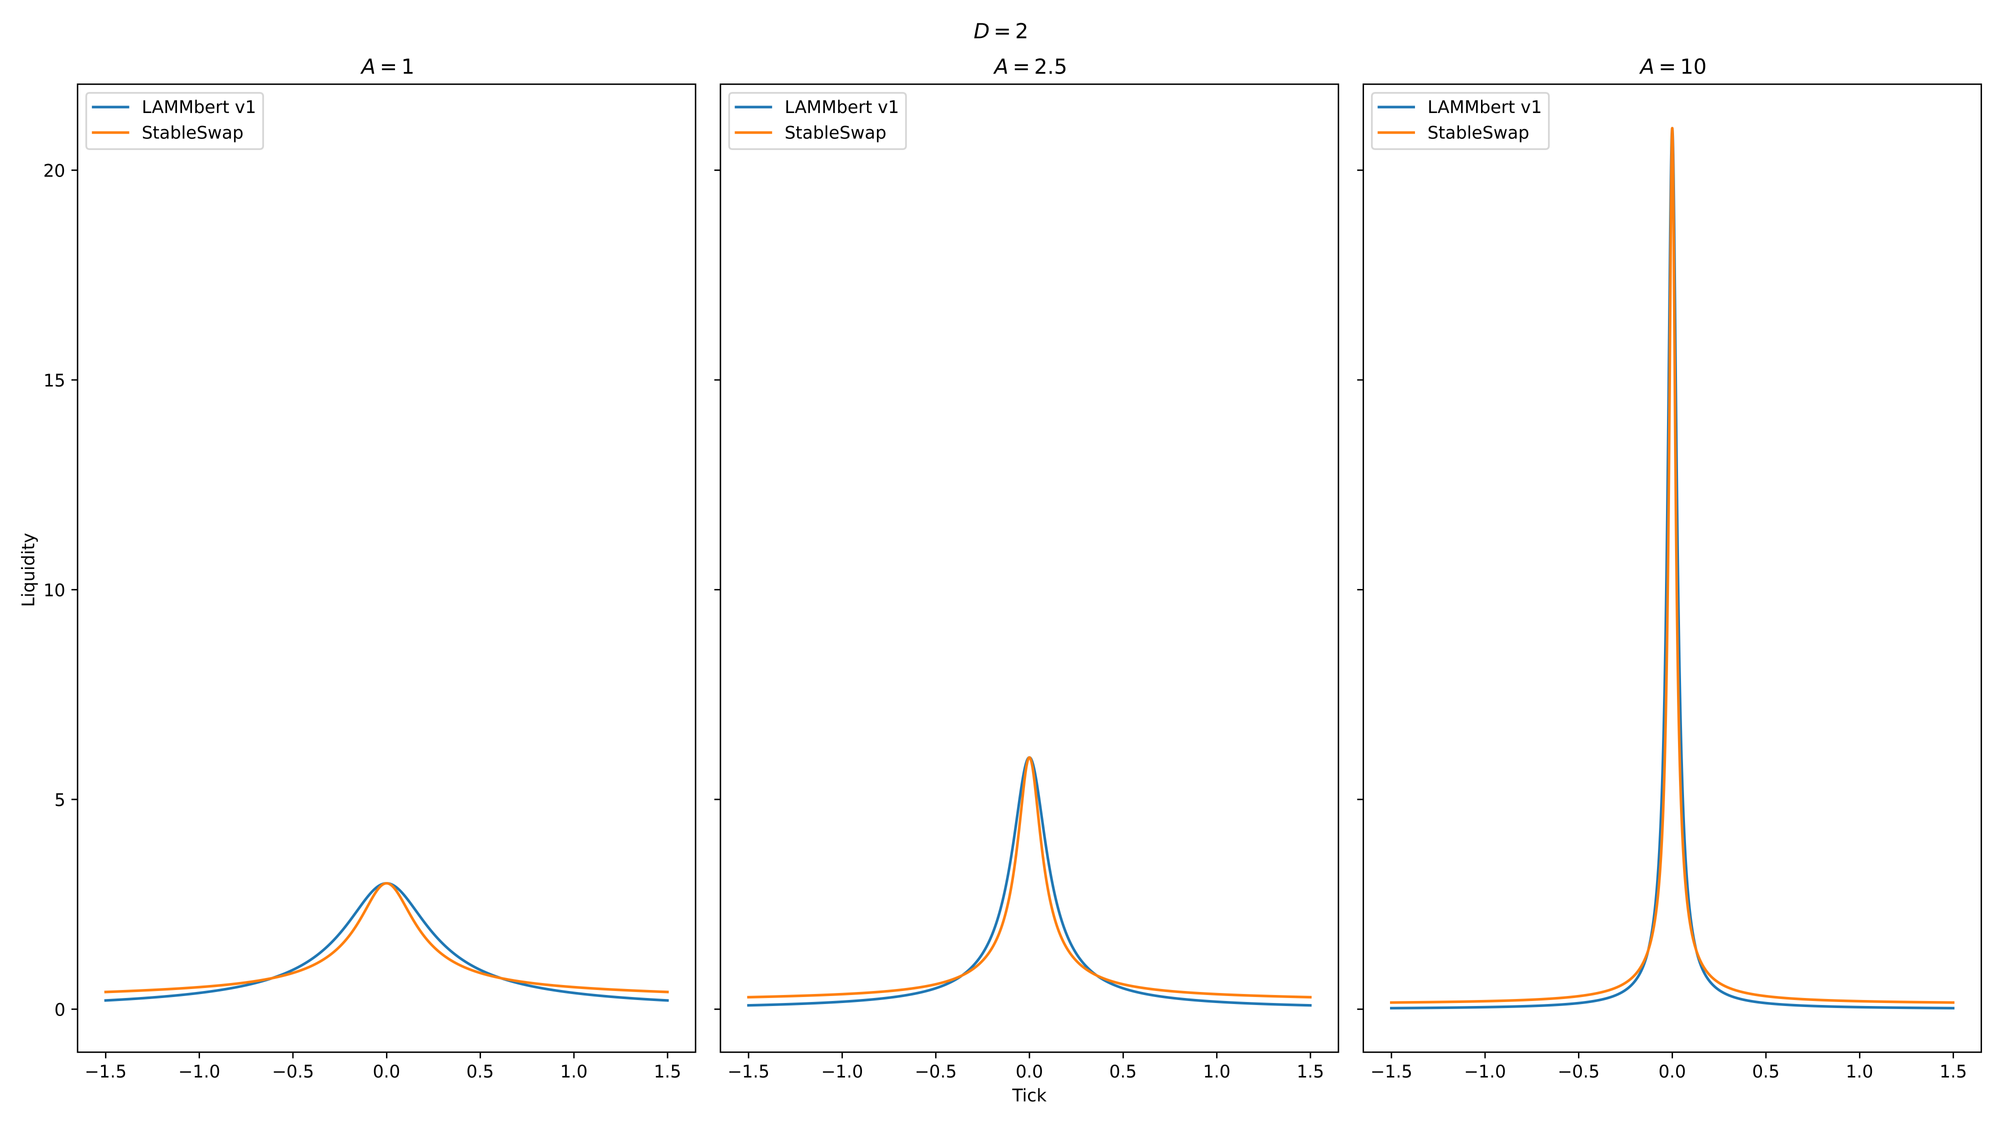
\includegraphics[width=1\linewidth]{figure1.png}
    \label{1}
\end{figure}

The two AMMs converge to each other as A becomes larger.

\textbf{LAMMbert v2}

$$\frac{32A\gamma^2p^2}{D^3}\cdot\frac{(y+xy')(px+y)xy}{\left(\gamma+1-\frac{4pxy}{D^2}\right)^3}+\frac{4A\gamma^2p}{D}\cdot\frac{(y+xy')(px+y)+(p+y')xy}{\left(\gamma+1-\frac{4pxy}{D^2}\right)^2}+p(y+xy')$$
$$=\frac{32A\gamma^2p}{D^2}\cdot\frac{y+xy'}{\left(\gamma+1-\frac{4pxy}{D^2}\right)^3}$$
$$y'=-\frac{\frac{32A\gamma^2p}{D^3}\cdot\frac{y(px+y-D)}{\left(\gamma+1-\frac{4pxy}{D^2}\right)^3}+\frac{4A\gamma^2}{D}\cdot\frac{p}{\left(\gamma+1-\frac{4pxy}{D^2}\right)^2}+\frac{1}{x}}{\frac{32A\gamma^2p}{D^3}\cdot\frac{x(px+y-D)}{\left(\gamma+1-\frac{4pxy}{D^2}\right)^3}+\frac{4A\gamma^2}{D}\cdot\frac{1}{\left(\gamma+1-\frac{4pxy}{D^2}\right)^2}+\frac{1}{y}}=-P=-e^t$$

\textbf{Curve v2}
$$\frac{32A\gamma^2p^2}{D^3}\cdot\frac{(y+xy')(px+y)xy}{\left(\gamma+1-\frac{4pxy}{D^2}\right)^3}+\frac{4A\gamma^2p}{D}\cdot\frac{(y+xy')(px+y)+(p+y')xy}{\left(\gamma+1-\frac{4pxy}{D^2}\right)^2}+p(y+xy')$$
$$=\frac{32A\gamma^2p^2}{D^2}\cdot\frac{(y+xy')xy}{\left(\gamma+1-\frac{4pxy}{D^2}\right)^3}+4A\gamma^2p\frac{y+xy'}{\left(\gamma+1-\frac{4pxy}{D^2}\right)^2}$$
$$y'=-\frac{\frac{32A\gamma^2p^2}{D^3}\cdot\frac{(px+y-D)xy^2}{\left(\gamma+1-\frac{4pxy}{D^2}\right)^3}+\frac{4A\gamma^2p}{D}\cdot\frac{(2px+y-D)y}{\left(\gamma+1-\frac{4pxy}{D^2}\right)^2}+py}{\frac{32A\gamma^2p^2}{D^3}\cdot\frac{(px+y-D)x^2y}{\left(\gamma+1-\frac{4pxy}{D^2}\right)^3}+\frac{4A\gamma^2p}{D}\cdot\frac{(px+2y-D)x}{\left(\gamma+1-\frac{4pxy}{D^2}\right)^2}+px}=-P=-e^t$$

Figure 2 is a visual comparison between two liquidity fingerprints.

\begin{figure}[H]
    \centering
    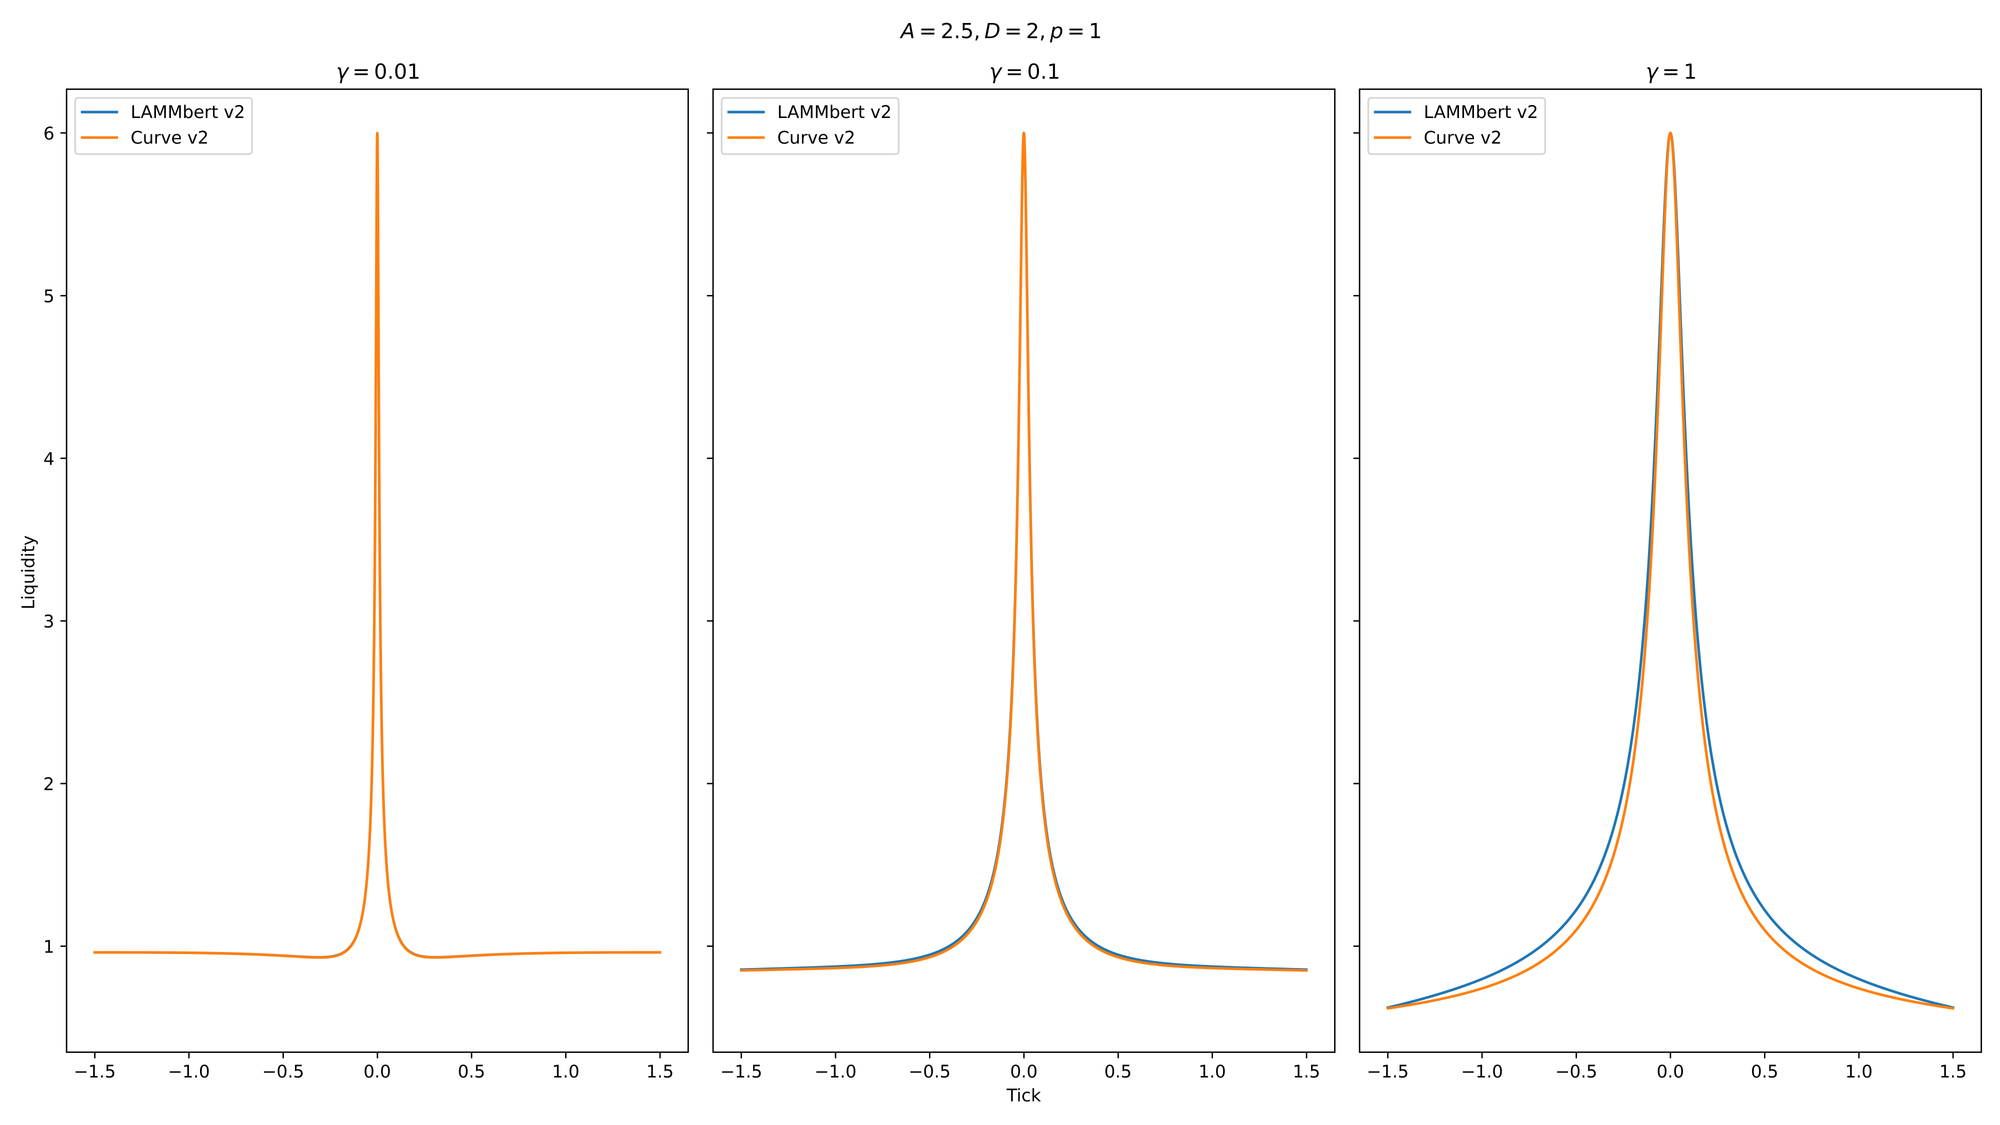
\includegraphics[width=1\linewidth]{figure2.png}
    \label{2}
\end{figure}

The two AMMs converge to each other as $\gamma$ becomes smaller. If the pegged price changes, the two AMMs will adjust liquidity concentration near the pegged price as you can see from Figure 3.

\begin{figure}[H]
    \centering
    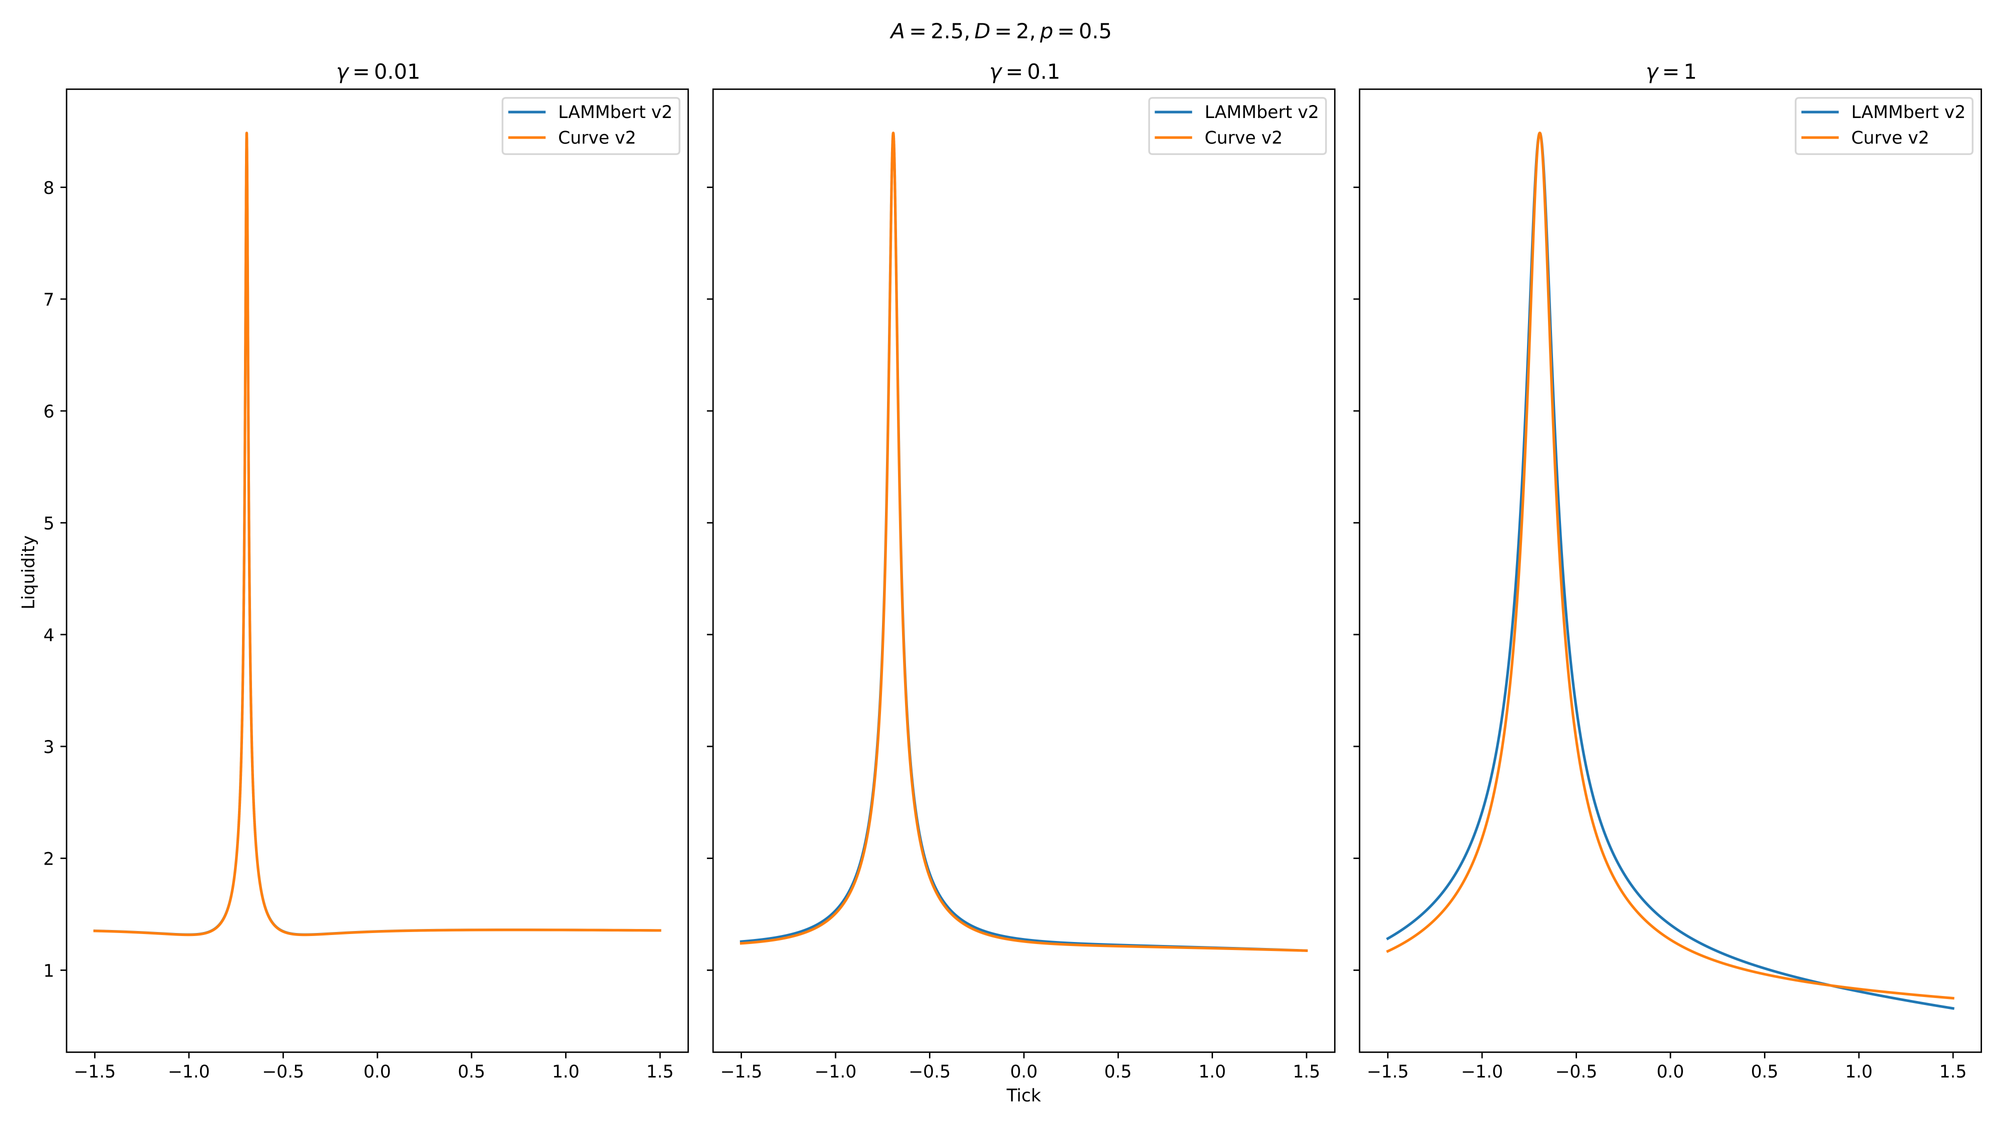
\includegraphics[width=1\linewidth]{figure3.png}
    \label{3}
\end{figure}

\end{document}
